%!TEX root = ../3dbook.tex

\setchapterpreamble[u]{\margintoc}

\graphicspath{{intro/}}
% \renewcommand*{\thelesson}{1.1}

\chapter{Introduction to 3D modelling of the built environment}%
\label{chap:intro}

% \fbox[0.8\linewidth][r]{\margintoc{}}

% 3D modelling and representations

The 3D modelling of the built environment involves the creation, manipulation and use of 3D digital representations of the real world, including buildings, terrains and infrastructure.
There are many approaches that can be taken with these representations, resulting in a huge variety of methods, each of them modelling things in a different way with different applications in mind.

% Breaking things down

When implemented in practice into a complete solution to a problem, these representations are not completely different from one another either.
Instead, they usually involve a unique mix of established techniques devised to represent shapes, connectivity and attributes.
The possible combinations of techniques means that the end result can differ greatly, but good solutions tend to strike a balance between their capabilities (\eg\ enough flexibility to model many types of objects), their simplicity (\eg\ using a consistent structure to allow for automated processing using simple rules) and how well they target the application they're used in.
In addition, the solutions that become widespread in practice also rely on many practical aspects, such as having good software support and widely available data.

% About the book

All of the above means that the representations used for 3D modelling of the built environment are interconnected and have many common elements.
Nevertheless, we have tried to split them into mostly independent chapters---each covering a different representation in detail.
The book starts from simple, generic and fundamental 3D modelling representations.
Then, it moves towards more complex ones that use others as building blocks and have more clearly defined applications within the built environment realm.
We focus mostly on the technical characteristics of each but also try to cover the most important practical aspects.
The book ends with chapters that tie the content to the creation of complex data sets through building reconstruction and to the application of the topics seen in the chapters.

% Contents

% how this process is split into a hierarchy working at different levels (from high to low).
% While the exact definition of these levels is a bit arbitrary, we follow a common model for geographic information, splitting them into spatial concepts, data models and data structures.
% We introduce each of these levels in its own section, including some basic examples for each.

% About the chapter

In this introductory chapter, we discuss the most important concepts that underlie the rest of the book and that should help the reader to tie the different chapters together.
These notions can be considered as a sort of glossary of the main ideas behind the 3D modelling of the built environment.

\section{Common conceptualisations of the 3D modelling process}

The 3D modelling process is quite complex, and is therefore usually described as more of a sequence of simpler processes that happen on multiple levels.
There are two common different conceptualisations for this in practice: a system of hierarchical abstractions that starts from the concrete real world and increasingly abstracts it into elements for a computer representation; or a series of steps that mimics the typical geoinformation process from measurements or acquisition, through one or more processing steps and ending with applications.

\subsection{Hierarchical abstractions}
\marginnote{hierarchical abstractions}\index{hierarchical abstractions}

One of the most useful concepts behind the 3D modelling of the built environment is that it is done through a series of abstractions of the real world, each working at a different abstraction level.
For instance, a typical high-level abstraction could divide the world into discrete objects (\eg\ individual buildings or plots of land), whereas a lower-level abstraction could divide each surface of a wall into triangles (\ie\ meshing) while satisfying certain characteristics (\eg\ minimum angles).
Each abstraction is thus an engineered partial solution to a complex modelling problem, which comes with its own technical choices, advantages and disadvantages, and applications for which it is suitable (or not).

For example, a 3D city model can be stored in a \texttt{.json} file where its entities are structured according to the CityJSON data model, with geometries represented as solids, and where each semantic surface is a triangulated mesh.
Alternatively, we can have a classified point cloud of the same city stored in an indexed series of \texttt{.las} files representing tiles.
Out of these two representations, the point cloud can be easily used as base elevation data or for many visualisation-based operations with comparatively little processing, but even simple spatial analysis operations (\eg\ counting the number of buildings or computing their volume) can be very complex.
On the other hand, the 3D city model could be used for complex spatial analysis operations (\eg\ wind and solar radiance simulations; Figure~\ref{fig:applications}), but some objects that are present in the real-world (\eg\ trees and fences) might be lost in the model or present only as artefacts.

\begin{figure}
\centering
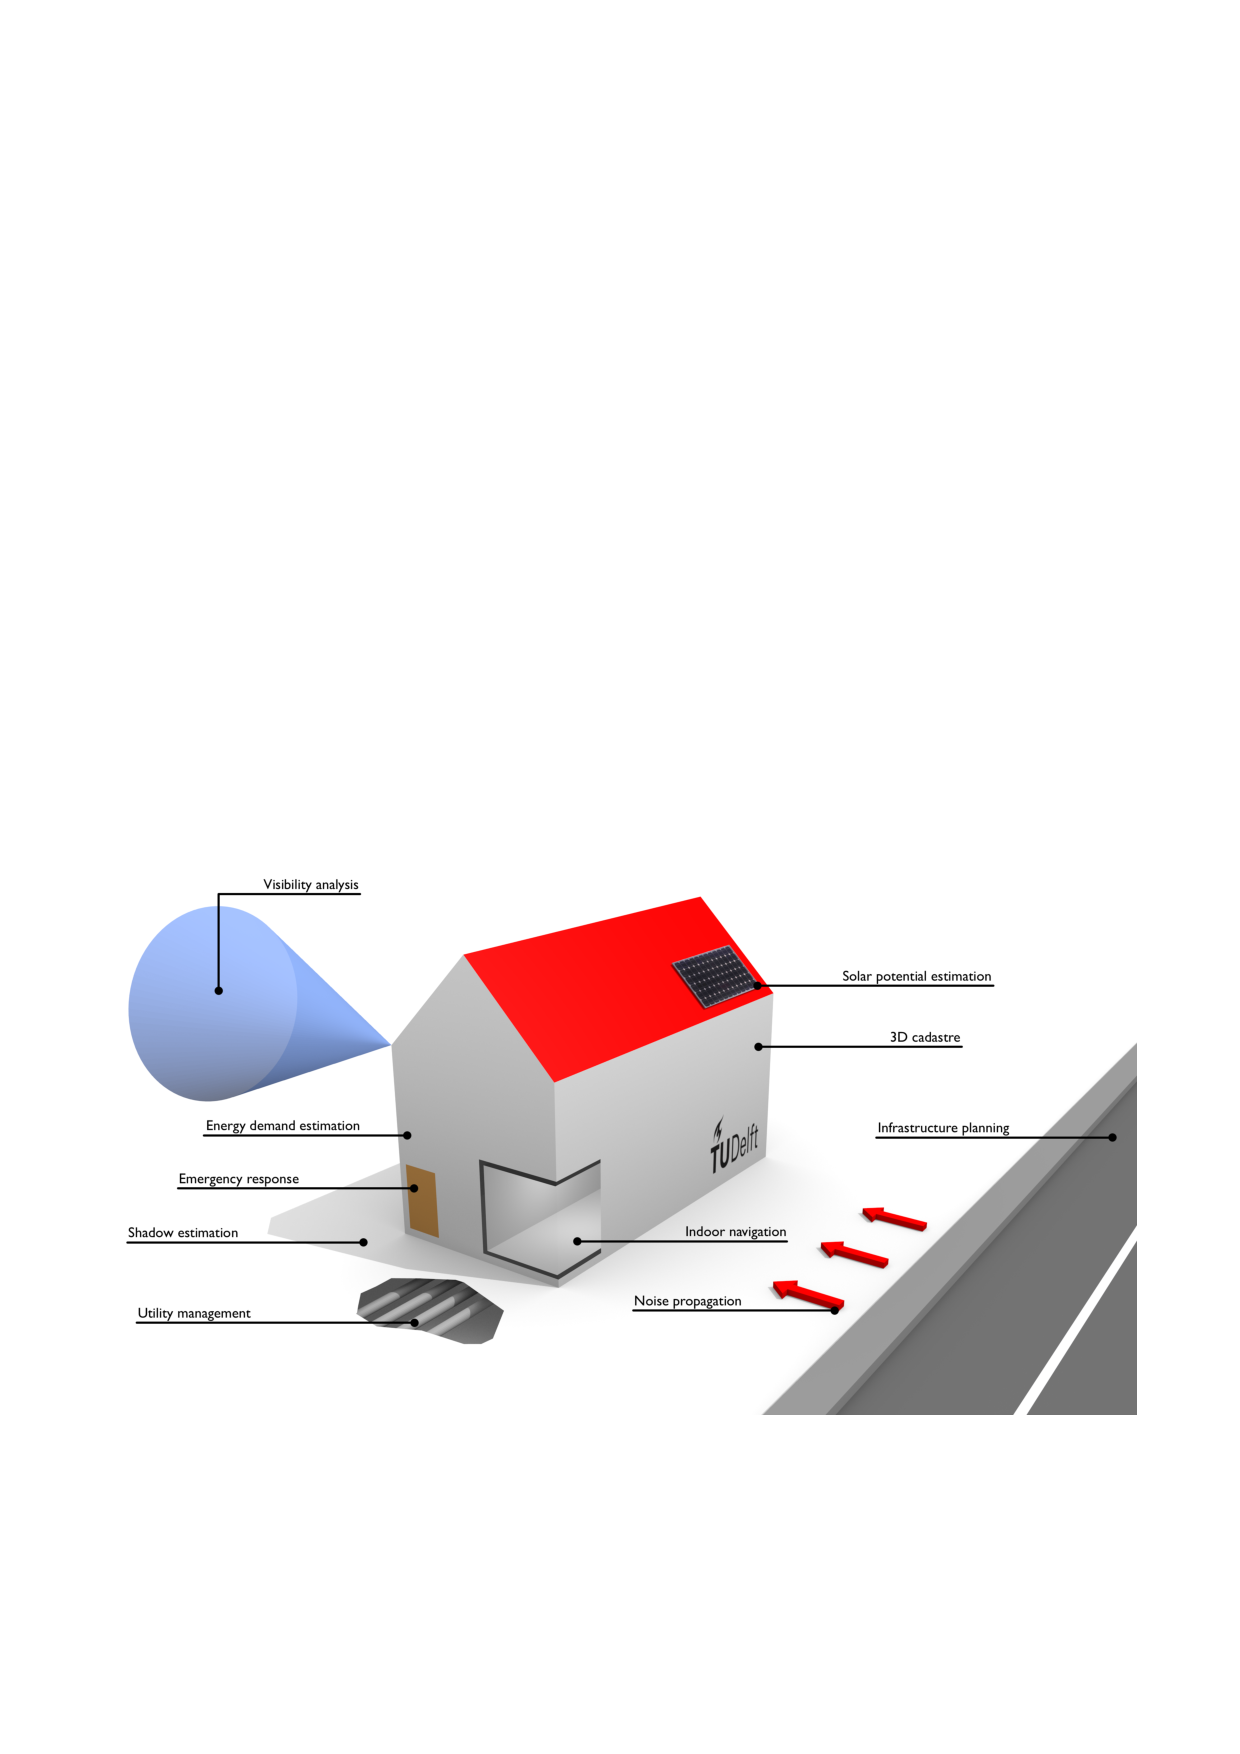
\includegraphics[width=\linewidth]{figs/applications.pdf}
\caption[Some typical applications of 3D city models]{Some typical applications of 3D city models~\citep{Biljecki15a}.}%
\label{fig:applications}
\end{figure}

\subsection{Geoinformation processing}

From a practical perspective, a common way to consider how space is structured is based on the usual steps in the geoinformation chain\marginnote{geoinformation chain}\index{geoinformation chain} (or pipeline).
This considers that one starts from the acquisition of data, either through traditional measurements (using anything from a tape measure to a total station) or using a variety of sensing technologies, including active methods using the reflections of electromagnetic waves (\eg\ all forms of lidar and radar) and vibrations (\eg\ underwater echo sounding and seismic methods), as well as passive methods (\eg\ digital images using any spectrum).

These `raw' measurements are then used to create simple primitives (\eg\ the points in a point cloud or the plane equation of a wall), and these are then further processed and assembled to create more complex 3D objects.

For instance, a typical process can go from a set of lidar full waveforms to a point cloud by deciding on appropriate return power thresholds, then to a series of meshes by reconstructing surfaces and fitting planes, and finally to a 3D city model with semantic surfaces by classifying and assembling the surfaces into 3D objects.
In every step of such a process, there is certain amount of information loss, but (ideally) the information that remains is more structured and meaningful.

\section{Geometry, topology and semantics}

Within the context of the built environment, 3D modelling is usually split into three different modelling components: geometry (modelling of shape), topology (modelling of connectivity) and semantics (modelling of qualitative or quantitative values).
These terms, as well as others covered in this section, are mostly derived from different branches of mathematics, but it is worth noting that their application within the geoinformation domain can differ substantially from their original mathematical meaning.
For instance, within geoinformation, it is common to refer to individual objects with a geometric description simply as \emph{geometries}, or to the interplay between different overlapping objects as \emph{a topology}.

\subsection{Geometry: Euclidean, Cartesian and point set}

When we model objects mathematically, we often rely on abstract geometric shapes, such as point, lines and planes.
The simplest mathematical descriptions for these are based on \emph{Euclidean geometry}\marginnote{Euclidean geometry}\index{Euclidean geometry}.
Euclidean geometry starts from a small set of geometric axioms considered to be intuitively obvious (Figure~\ref{fig:line}).
Using these axioms, it is possible to construct more complex objects (\eg\ a triangle covering the area between three points) and to define properties, such as relative distances, angles and areas.
However, objects in Euclidean geometry do not have an absolute position in space.

\begin{marginfigure}
\centering
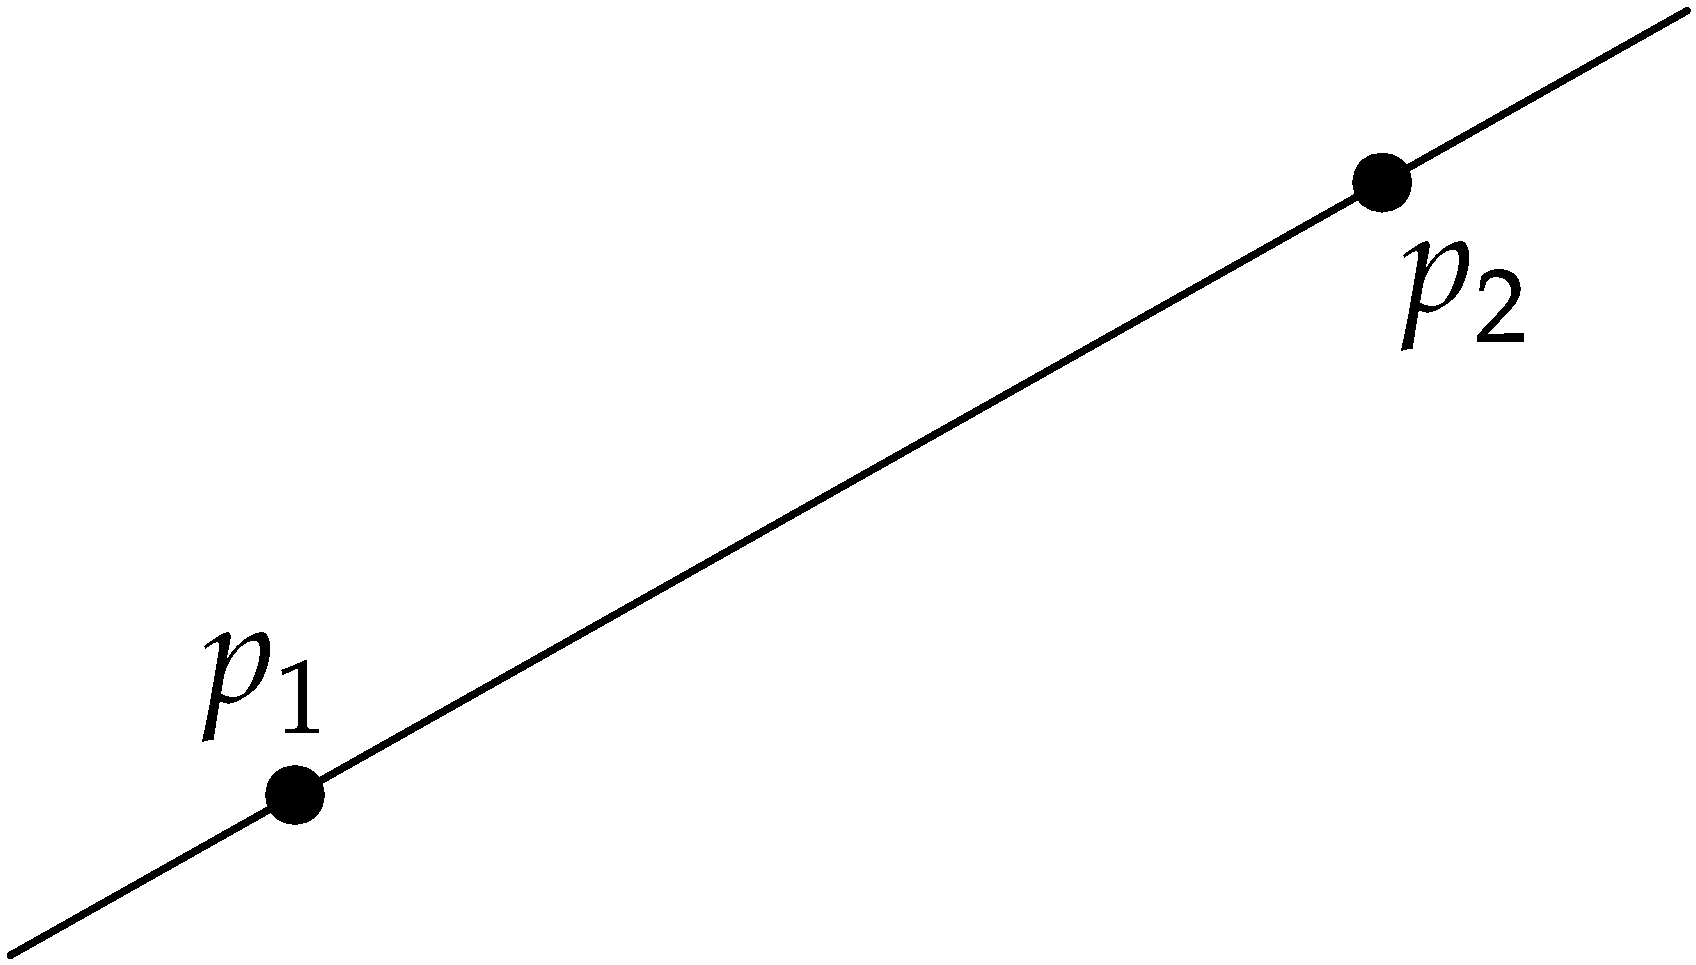
\includegraphics[width=\linewidth]{figs/line.pdf}
\caption[Two points can be used to describe a line in Euclidean geometry]{Since there is exactly one line that passes through any pair of points, two points can be used to describe a line in Euclidean geometry.}%
\label{fig:line}
\end{marginfigure}

Where this notion is required, analytic or \emph{Cartesian geometry}\marginnote{Cartesian geometry}\index{Cartesian geometry} adds the concept of coordinates to the objects of Euclidean geometry, which makes it possible to uniquely describe the absolute location of a point (Figure~\ref{fig:point}), the length of a line or the angle between two lines.
This analytic description also makes it possible using algebra to compute the exact value of some properties, such as the distance between two points (as described by their coordinates).

\begin{marginfigure}
\centering
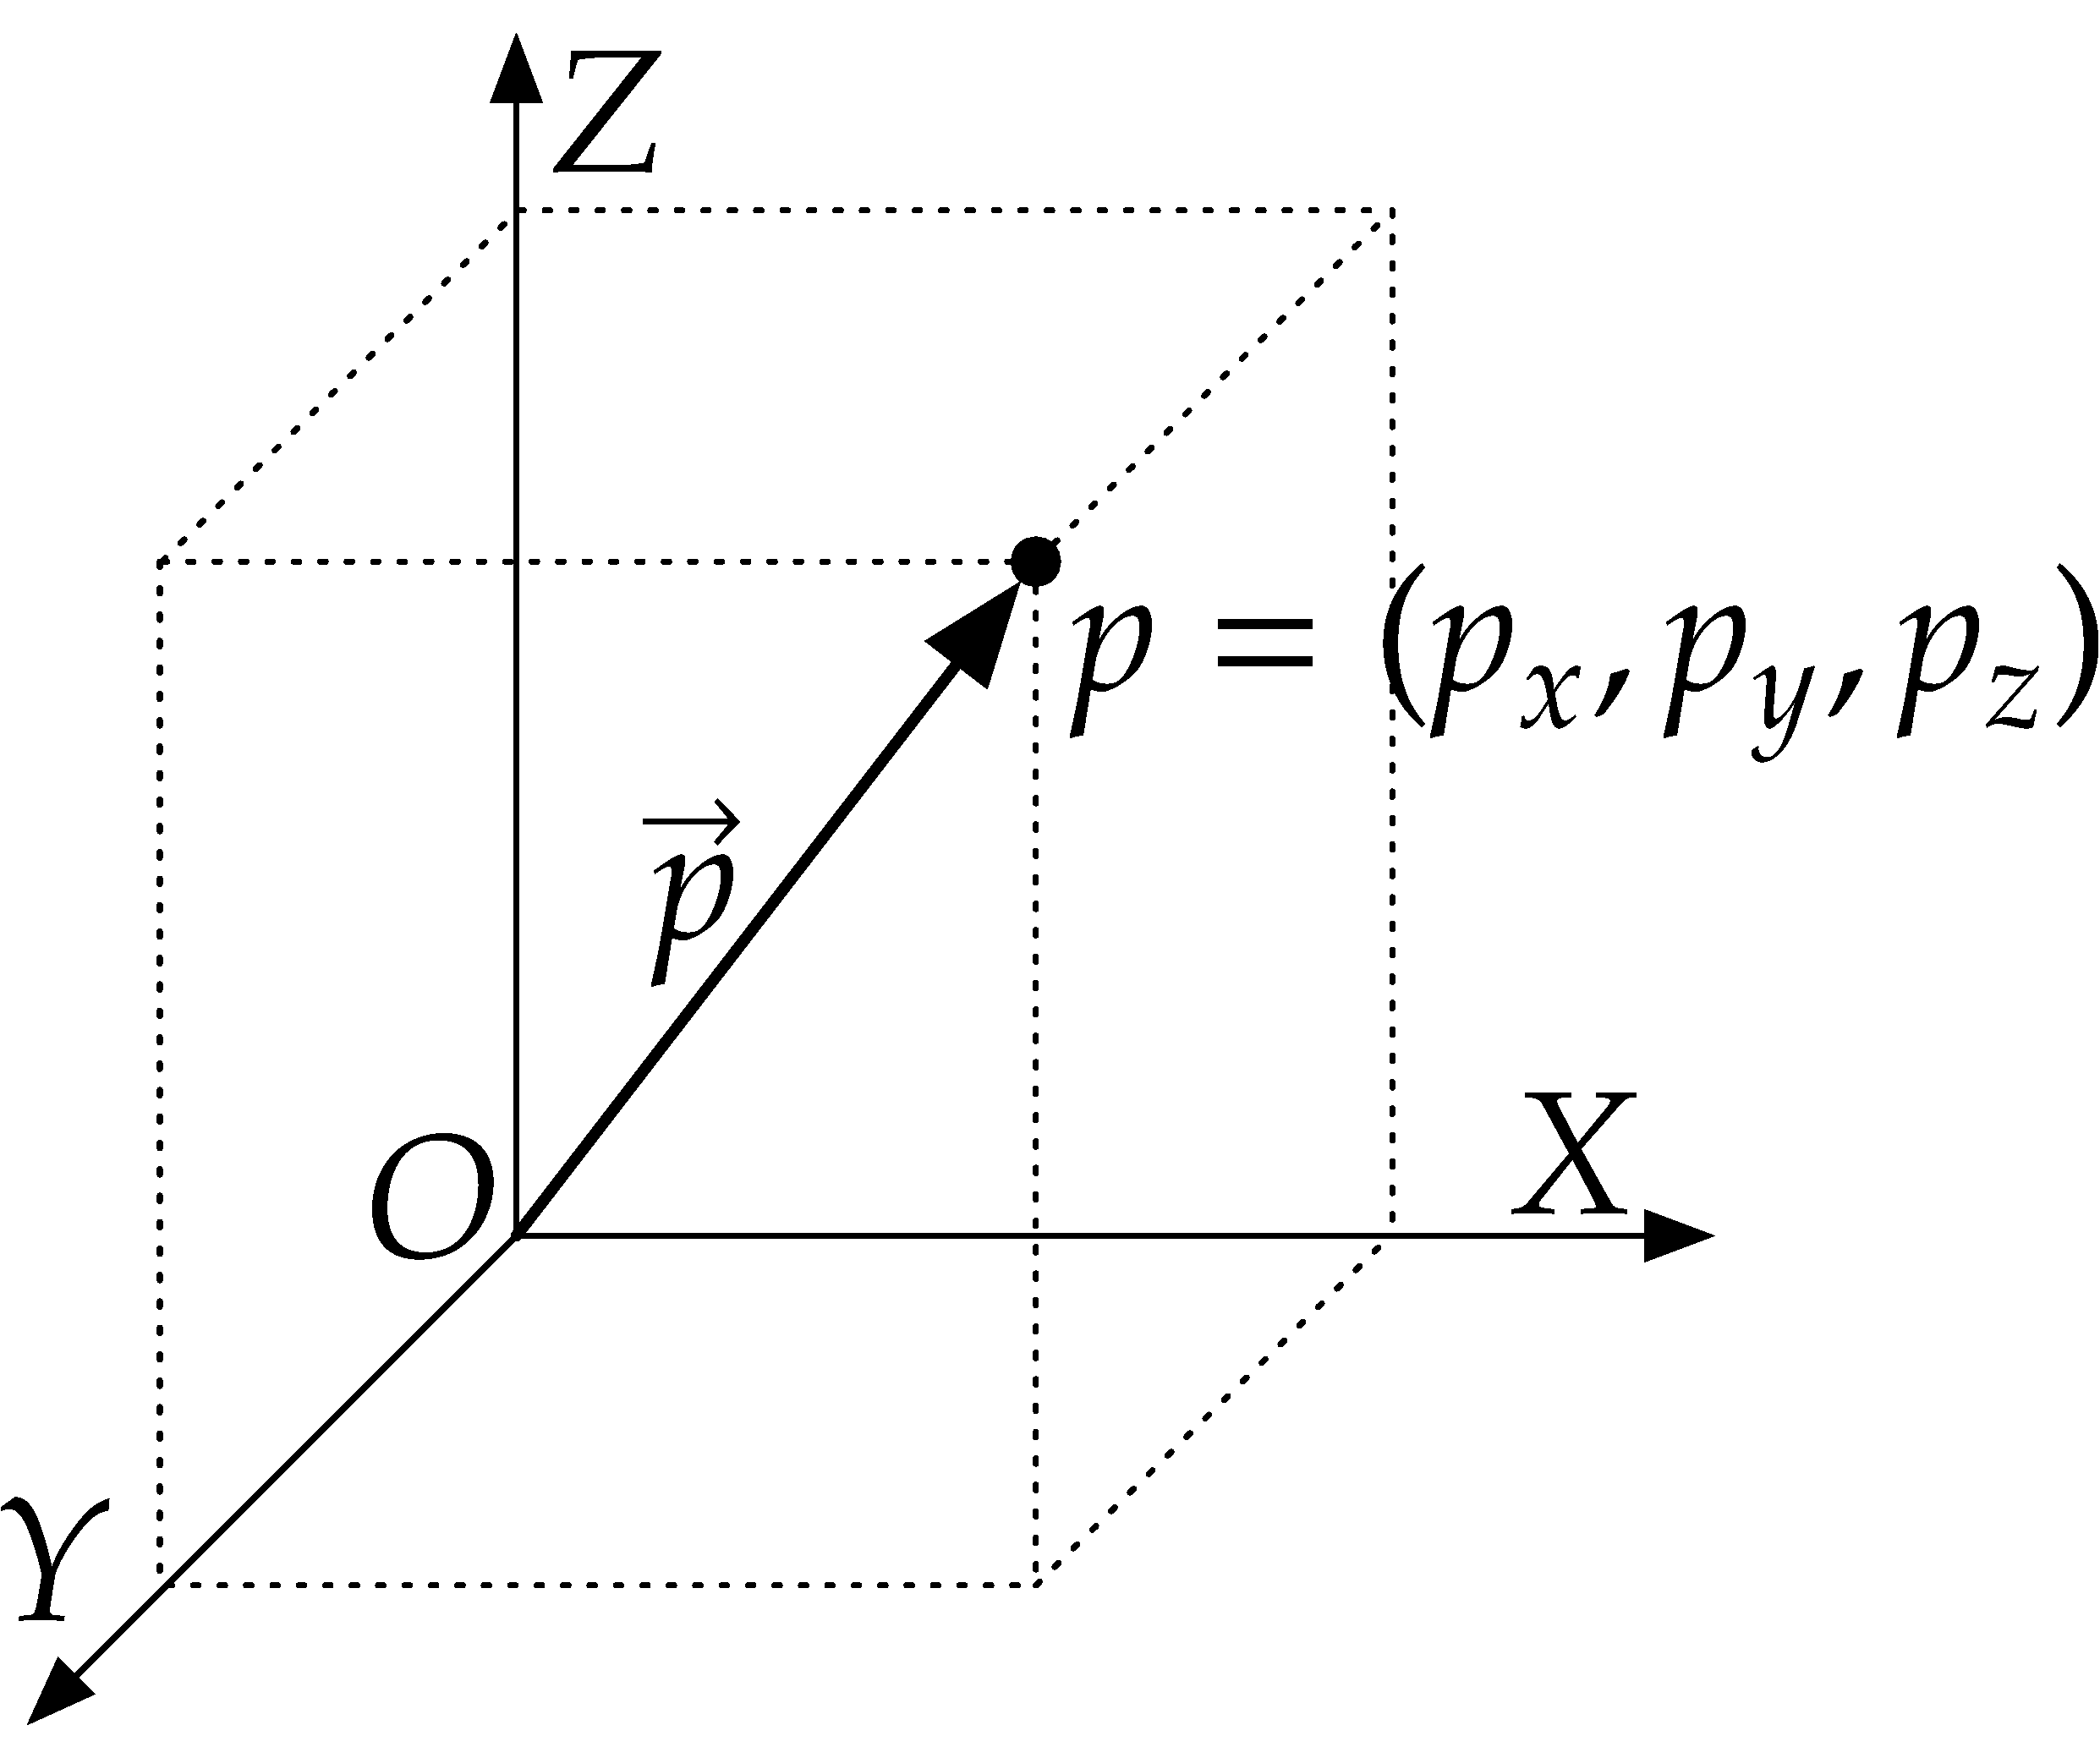
\includegraphics[width=\linewidth]{figs/point.pdf}
\caption[A point in 3D described by an ordered list of three coordinates]{A point in 3D described by an ordered list of three coordinates $(p_x,p_y,p_z)$.}%
\label{fig:point}
\end{marginfigure}

Pure analytical solutions can be however tricky (\eg\ points placed at irrational values), so some other definitions used for modelling objects rely on \emph{point set geometry}\marginnote{point set geometry}\index{point set geometry}.
This method uses the mathematical definitions of sets and of operations between sets to define objects as sets of (often infinitely many) points.
For instance, we can say that a sphere is a point set where the distance to a given point (\ie\ the centre) is equal to a value, or to define an object as the intersection between two other objects.

% \begin{figure}[htbp]
% \centering
% \begin{subfigure}[b]{0.45\linewidth}
% 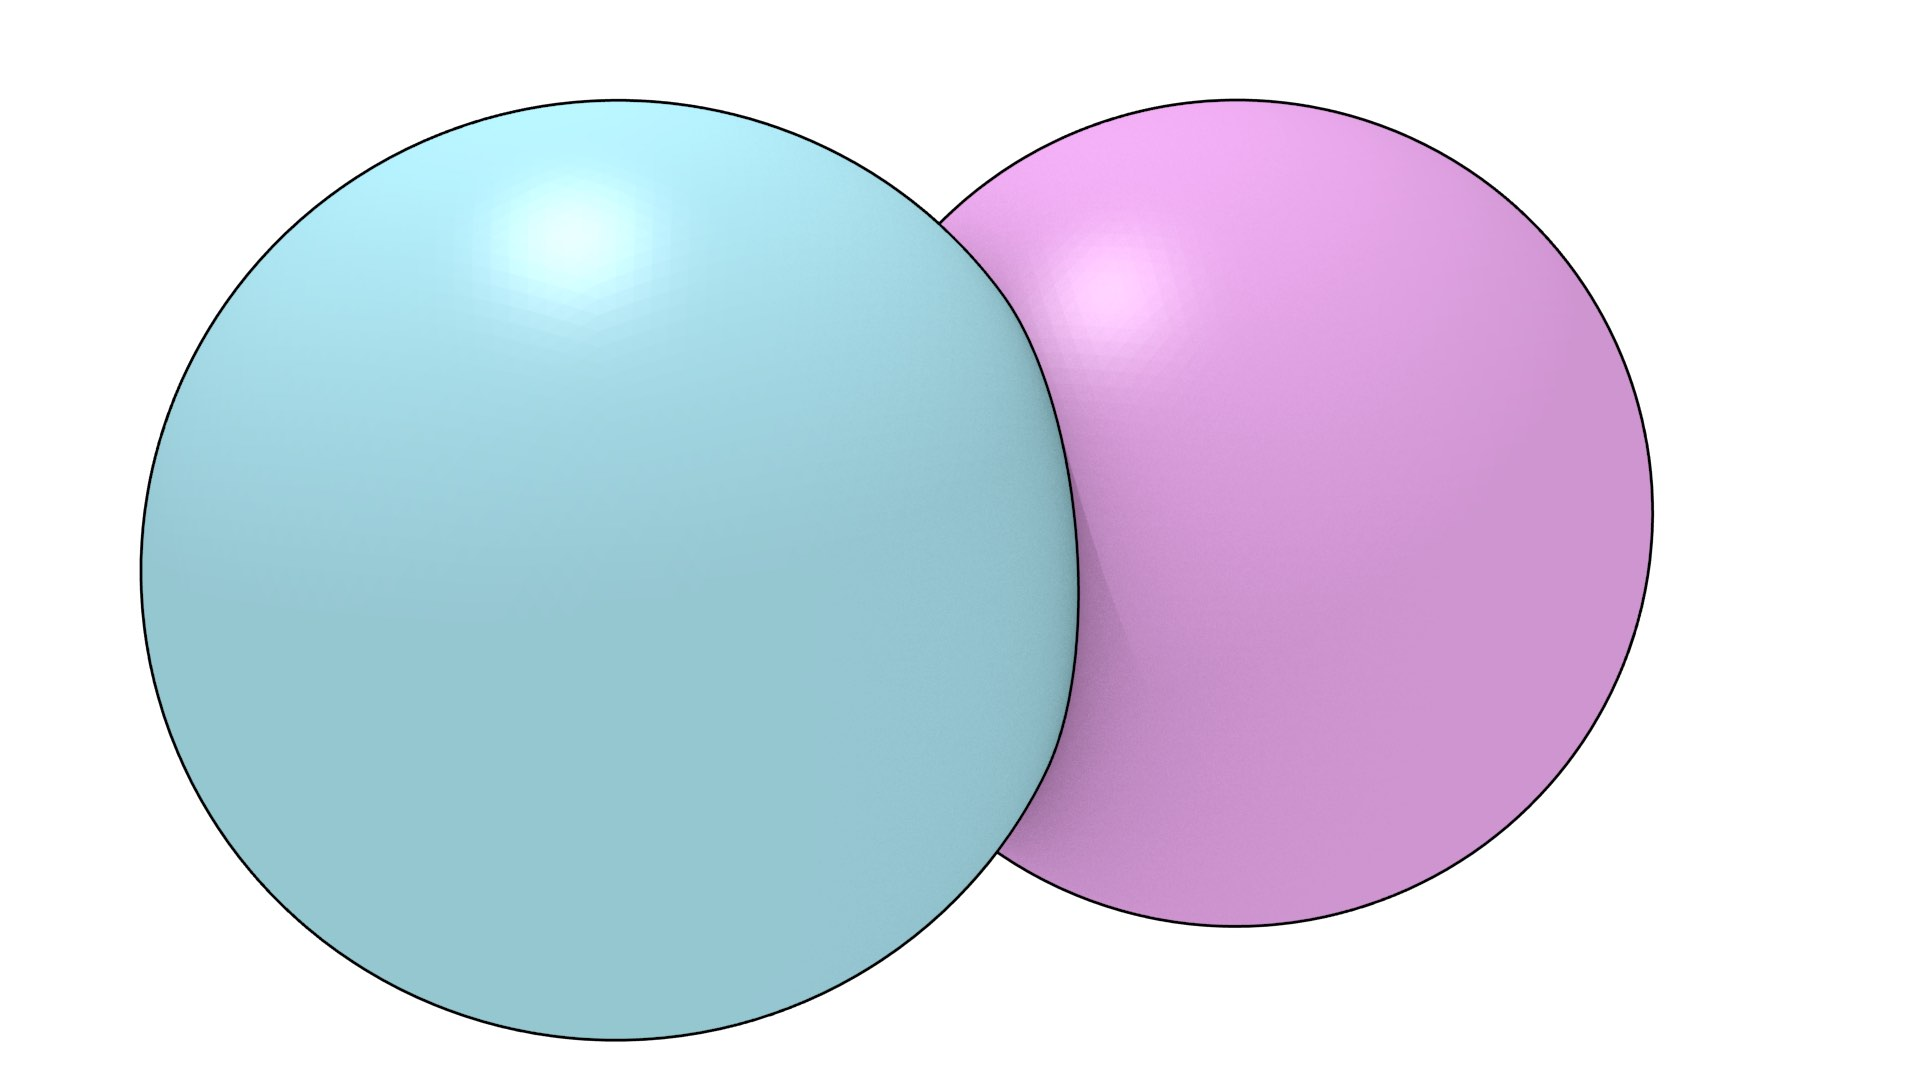
\includegraphics[width=\linewidth]{figs/boolean}
% \caption{$\mathbb{A}$ (purple) and $\mathbb{B}$ (blue)}%
% \label{subfig:boolean}
% \end{subfigure}
% \begin{subfigure}[b]{0.45\linewidth}
% 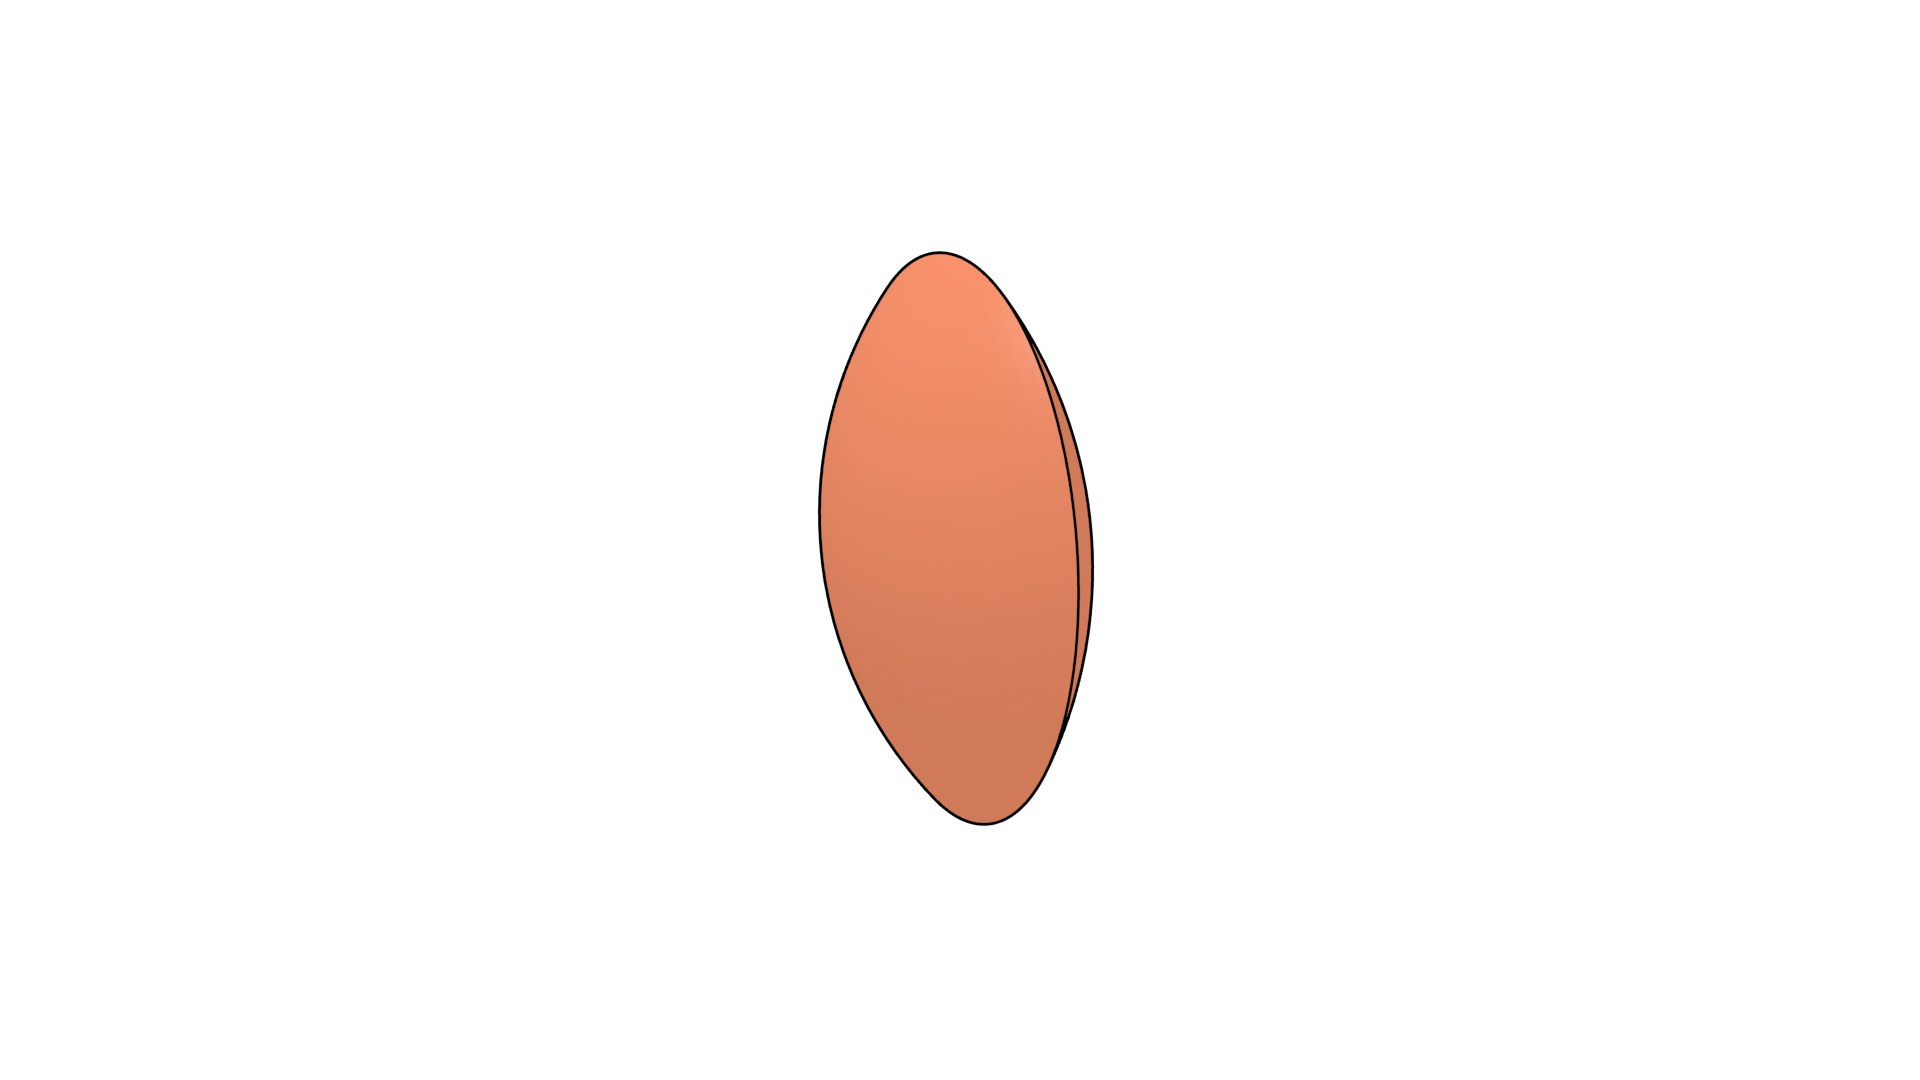
\includegraphics[width=\linewidth]{figs/boolean-intersection}
% \caption{Intersection: $\mathbb{A} \cap \mathbb{B}$}%
% \label{subfig:boolean-intersection}
% \end{subfigure}
% \caption{Based on two balls $\mathbb{A}$ and $\mathbb{B}$, other objects that can be defined using Boolean set operations using point set geometry.}%
% \label{fig:boolean}
% \end{figure}

Within the context of the built environment, all of these types of geometric descriptions are used to define 3D objects.
Euclidean geometry is what is most often used to describe geometric primitives, Cartesian geometry is usually used to append coordinates to points or equations to more complex shapes, and point set geometry is the basis for the representations that are based on implicit geometries.

\subsection{Explicit and implicit geometry}

Another distinction with respect to geometry is between \emph{explicit} and \emph{implicit} geometries.
This separation is related to the notion of \emph{explicit} and \emph{implicit functions} or \emph{equations} in mathematics.
The exact definitions are a bit tricky, as a simple approximation, explicit functions between variables can express one variable in terms of the others, whereas implicit functions cannot, or at least cannot do so easily.
Instead, they tend to be defined more indirectly using additional variables or based on conditions that all variables need to jointly comply with.

Within the context of 2D/3D modelling, \emph{explicit representations of geometry}\marginnote{explicit geometry}\index{explicit geometry} are those that are more direct, usually using more straightforward descriptions of point coordinates or the equations typically used to describe shapes, \eg\ lines, planes or polygons.
Complex objects are usually described explicitly using a large number of simple primitives.

Meanwhile, \emph{implicit representations}\marginnote{implicit geometry}\index{implicit geometry} are those that rely on more indirect descriptions, such as sequences of operations or complex functions, which often rely on non-spatial parameters (\ie\ not \(x\), \(y\) or \(z\)).
Usually, some complex objects can be described implicitly using only a few primitives.
Many more advanced geoinformation processing methods rely on the specific properties of a certain type of implicit geometries.

However, since many methods and software rely on explicit geometries, obtaining explicit geometries from implicit ones is a common task.
It can be quite difficult in practice, often involving difficult calculations or leading to problems of discretisation or loss of precision.

\subsection{Topology: graphs and algebraic topology}

The concepts from different branches of geometry are useful to describe the overall shape of objects, but in practice we often need to add concepts of topology as well.
For instance, this is often used to describe relationships between objects, such as adjacency or connectivity.
In the 3D modelling of the built environment, topology is especially important because the standard approach to model complex objects is to divide them into small elements, and thus we also need to describe how these elements are connected.

In its simplest form, topology often takes the form of a \emph{graph}\marginnote{graph}\index{graph}, where the elements are vertices that are connected by (directed) edges.
Vertices often correspond to geometric points and edges to geometric line segments, but this is not always the case.
For instance, in a \emph{dual}\marginnote{duality}\index{duality} representation, vertices can correspond to polygons and the edges connecting them can correspond to the connections between adjacent polygons.

\emph{Algebraic topology}\marginnote{algebraic topology}\index{algebraic topology} takes the concept of a graph further by allowing us to use higher-dimensional objects (\eg\ faces and volumes), which will be used to describe simplices and cells in some of the data models that we will discuss later in the course.
It also makes it possible to describe objects based on sets, as well as to create operations that modify these sets.

\section{Objects and fields}

From a theoretical GIS standpoint, the typical way to conceptualise space recognises two ways of looking at the world: \emph{objects} and \emph{fields}.
The objects\marginnote{object}\index{object} view considers that space is empty and is populated by discrete objects.
In order to represent this view, objects are therefore modelled individually (\eg\ a building modelled as a set of surfaces), although it is worth noting that these objects can be smaller or bigger depending on the level of detail involved.
For instance, a building information model can model every individual brick, fire suppression sprinkler or layer of insulation in a wall as separate objects with high detail; whereas national or city-wide models can aggregate or generalise multiple buildings into simple rectangular city blocks.

% TODO: more about objects
% Mathematically, the representation of objects takes a few different forms.
%  specifying which object(s)

By contrast, the fields\marginnote{field}\index{field} view considers that there are certain attributes that fill regions of space and have a changing value as one moves through it.
The typical examples are physical characteristics, such as the elevation of a terrain, the temperature or the wind speed.
Since we generally cannot know or store the values of fields in every possible location, of which there might be infinitely many, the standard approach is to mathematically model an approximation (\eg\ elevation modelled as an interpolated set of points).

% Mathematically, a field is usually defined as a model of the spatial variation of an attribute over a spatial domain.
% , we assume this domain to be $\mathbb{R}^d$, the $d$-dimensional Euclidean space.
% It is modelled by a function mapping one point $p$ in $\mathbb{R}^d$ to the value of $a$, thus 
% \[
%   a = f(p)
% \]
% The function can theoretically have any number of independent variables (\ie\ the spatial domain can have any dimensions), but in the context of geographical phenomena the function is usually bivariate \((x,y)\) (\eg\ for the elevation of terrain) or trivariate \((x,y,z)\) (\eg\ for the temperature of a body of air).

%

The representation of both objects and fields in a computer faces many common problems. 
Foremost, objects and fields are both continuous, and, by contrast, computers are discrete machines. 
They must therefore be acquired in a discrete way, \eg\ measuring fields through samples or measurements from sensors, or acquiring the geometry of objects through a limited number of measured or remotely sensed points.

This discrete acquissition process is affected by the acquisition tools and techniques, and is made more complex because we seldom have direct access to the whole object of interest, either due to physical or cost limitations.
For example, to collect field samples in the ground, we must dig holes or use other devices (\eg\ ultrasound penetrating the ground); underwater samples are collected by instruments moved vertically under a boat, or by automated vehicles; and samples of the atmosphere are collected by devices attached to balloons or airplanes.
Similarly, buildings and infrastructure can be acquired through images captured from a limited number of pictures from a few angles, using cameras with a limited resolution and often resulting in parts that are not sensed clearly or missing altogether.

Then, it is necessary to reconstruct objects or fields from these limited samples using different discrete techniques.
% Moreover, because of the way they are collected, geoscientific datasets often have a highly sparse and anisotropic distribution, the distribution can be for instance dense vertically (with a sample every 2m in that real-world case) but extremely sparse horizontally (water columns are located at about 35km from each others).

\section{Data models and data structures}

A data model\marginnote{data model}\index{data model} is a high-level formalised way to structure information, generally using a set of abstract classes, relationships between them, and attributes to store information about them.
In the context of geomatics, these classes are often spatial representations of real-world objects.
Some aspects that are typically defined by a data model include the kind of discretisation of space that is used (\eg\ a grid) and the formal mathematical bases of the model (\eg\ describing the basic elements of a data model as tuples).
Certain data models also include formalised operations that can be performed on their defined classes.

Data models are deliberately ambiguous and far from a computer representation, and so implementing them involves various engineering decisions and can be tricky.
Moreover, without some specific encoding rules, different people will make different engineering decisions and thus likely implement a data model very differently.

The typical examples of data models used in (older) geomatics literature are the \emph{raster}\marginnote{raster}\index{raster} and \emph{vector}\marginnote{vector}\index{vector} data models.
These examples are historically accurate because they are clear-cut high-level descriptions that can each be implemented in a variety of ways.
For instance, rasters can be encoded by traversing them in a given order and listing the values in each cell one by one (known as exhaustive enumeration), by splitting it into successive halves of a uniform value using a $k$-d tree, or by compressing it using a Wavelet transform (\eg\ in JPEG 2000 images).

However, it is worth noting that nowadays the term data model is most often used to refer to highly complex abstractions of the real world that are suitable for a particular domain.
These can include a mixture of geometric, topological and semantic components.
Data models are often available in the form of a \emph{schema}\marginnote{schema}\index{schema}---a descriptive document that specifies the data model in a formal manner.
Schemas are often described using UML models (\eg\ CityGML; Figure~\ref{fig:citygml}), although using a computer-processable language (\eg\ JSON schema in CityJSON, EXPRESS in IFC, XSD in CityGML) is generally better since it allows processing the schema, such as for validation.

\begin{figure*}
\centering
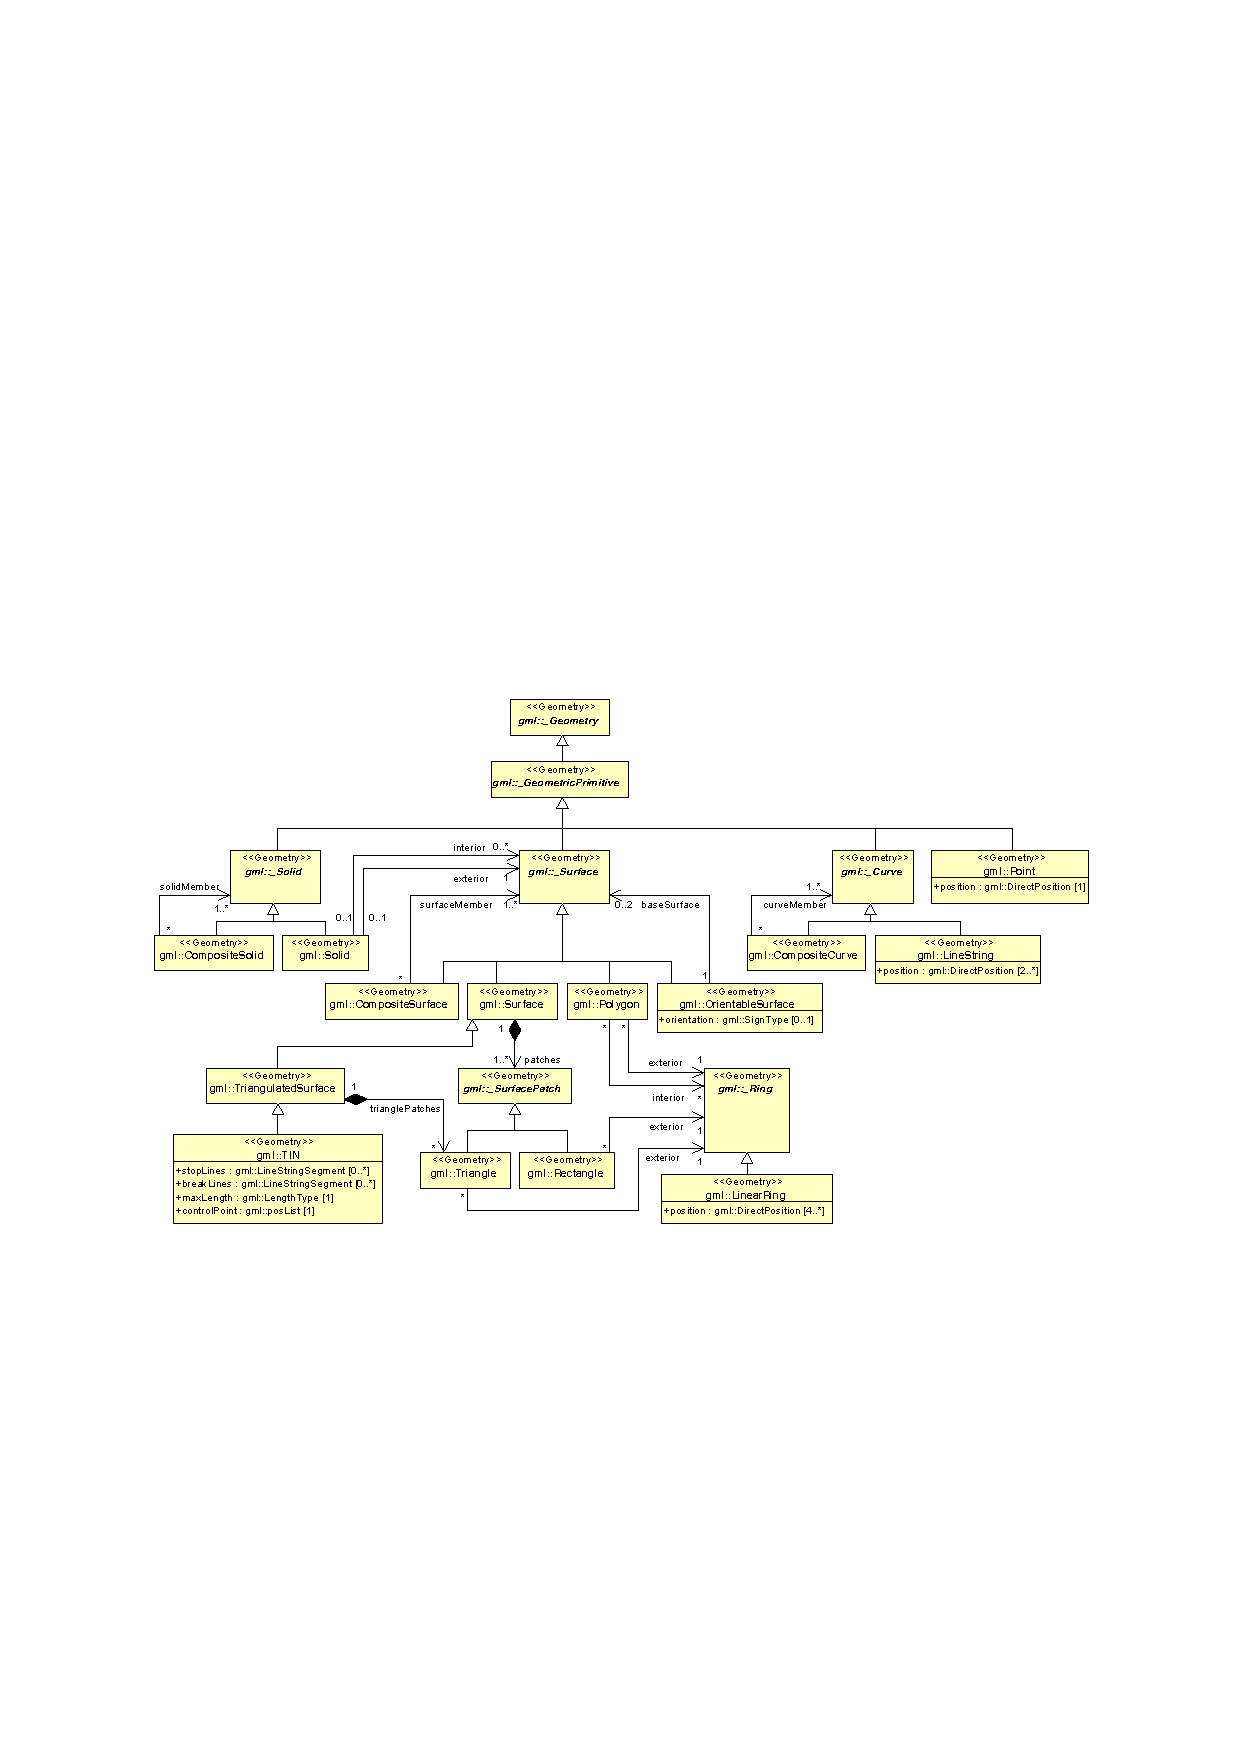
\includegraphics[width=\linewidth]{figs/citygml.pdf}
\caption[The geometry classes used in the CityGML 2.0 standard]{The geometry classes used in the CityGML 2.0 standard~\citep{CityGML2.0}.}%
\label{fig:citygml}
\end{figure*}

A data structure\marginnote{data structure}\index{data structure} is a low-level description that specifies how to implement a data model, or occasionally a combination of multiple data models.
Data structures are defined with little to no ambiguity, specifying features such as what sort of storage should be used for a given primitive (\eg\ an array or a linked list). 
As opposed to a data model, creating a computer implementation of a data structure is thus relatively straightforward, and different people implementing the same data structure will end up with very similar implementations.

Data structures can be specified using the same methods as data models, \eg\ UML models, but more explicit descriptions are also possible.
For example, database tuples or table definitions in SQL can be used when a database implementation is expected, or snippets of source code  (generally in the style of the C programming language) can be used when it is expected to be used in memory.

Following a typical example, if we assume that we are implementing a standard vector data model with polygons, we could choose to do so using a half-edge data structure (Figure~\ref{fig:halfedge-2}).
Note that the low-level definition of a half-edge pretty much defines the structure of its computer implementation.

\begin{marginfigure}
\centering
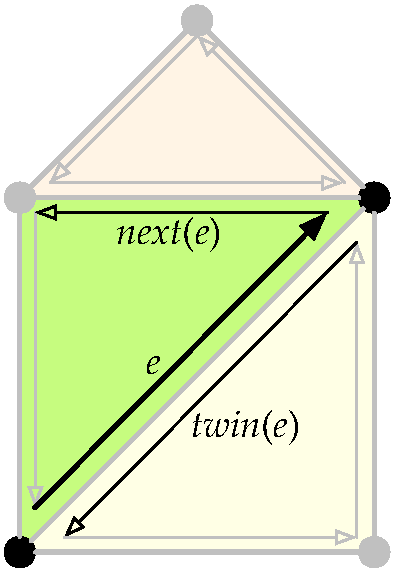
\includegraphics[width=\linewidth]{figs/halfedge-2.pdf}
\caption[The half-edge data structure]{The half-edge data structure can store sets of polygons based on elements known as half-edges, which represent an edge within a face.
A half-edge \(e\) is related to two vertices (the origin and the destination) and one face, and is linked to its next half-edge (on the same face) and its twin half-edge (on the adjacent face).}%
\label{fig:halfedge-2}
\end{marginfigure}

%%%
%
\section{Exercises}

\begin{enumerate}
  \item Do the levels of the hierarchy in the `hierarchical abstractions' model correspond to the steps in the `geoinformation chain'?
	\item What is noisier: the `raw' measurements in the early steps of the geoinformation chain, or the more processed products of the last steps.
	\item Give an example of a field that is not a natural physical characteristic.
	\item Consider whether a point cloud is a data model or a data structure. If it is a data model, what sort of data structure could be used to represent it?
  \item What is the relationship between the `hierarchical abstractions' model and the concepts of data models and data structures?
	% \item Describe an alternative data structure that can be used to represent the vector data model (\ie\ not the half-edge data structure). What are some advantages/disadvantages of each data structure?
\end{enumerate}



%%%
%
\section{Notes and comments}

% \citet{Frank92} is the original source that divides representations into spatial concepts, data models and data structures.
% It is partly out of date since it long predates the semantic data models that are used nowadays, but it is still a good paper, and a precursor to the ones we described here.

Chapter 2 of Ken's PhD thesis\marginnote{\faExternalLink\ \url{https://3d.bk.tudelft.nl/ken/en/thesis/math.html}} describes all the mathematical notions from this chapter in a bit more detail.
Section 3.1\marginnote{\faExternalLink\ \url{https://3d.bk.tudelft.nl/ken/en/thesis/modelling-background.html\#se:spatial-modelling}} lists many data models and data structures with references to the original papers where they came from.

\citet{Couclelis92} is the original source that clearly formalised the difference between objects and fields.
\citet{Goodchild92} links objects and fields to specific computer models that are suitable for them.

\citet{Mantyla88} has an excellent overview of different 3D representations.
Some other good standard alternatives are \citet{Requicha80,Hoffmann92,Foley95}.
A newer book freely accessible from the campus is \citet{Salomon11}.

